\chapter{Methodology and Development Process}

\section{Development Methodology}

\subsection{Agile Development Approach}

VIRASAT was developed using an iterative, feature-driven approach inspired by Agile methodologies:

\begin{enumerate}
    \item \textbf{Sprint Planning}: Features broken down into manageable tasks
    \item \textbf{Incremental Development}: Core features built first, then enhanced
    \item \textbf{Continuous Integration}: Regular testing and integration of new features
    \item \textbf{Iterative Refinement}: User feedback incorporated into subsequent iterations
\end{enumerate}

\subsection{Development Phases}

\begin{figure}[H]
\centering
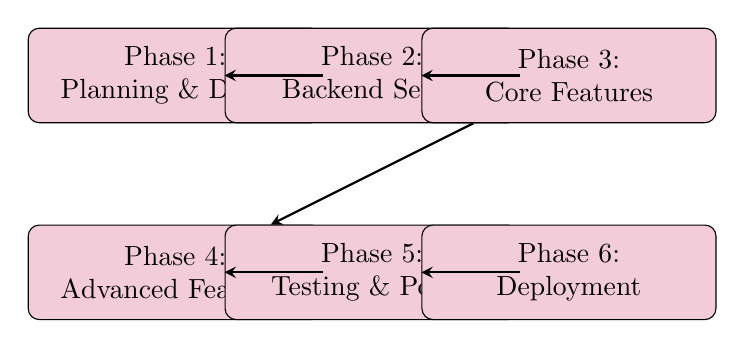
\begin{tikzpicture}[
    node distance=2.5cm,
    phase/.style={rectangle, draw, fill=purple!20, text width=3.5cm, text centered, rounded corners, minimum height=1.2cm},
    arrow/.style={->, >=stealth, thick}
]

\node[phase] (phase1) {Phase 1:\\Planning \& Design};
\node[phase, right of=phase1] (phase2) {Phase 2:\\Backend Setup};
\node[phase, right of=phase2] (phase3) {Phase 3:\\Core Features};
\node[phase, below of=phase1] (phase4) {Phase 4:\\Advanced Features};
\node[phase, right of=phase4] (phase5) {Phase 5:\\Testing \& Polish};
\node[phase, right of=phase5] (phase6) {Phase 6:\\Deployment};

\draw[arrow] (phase1) -- (phase2);
\draw[arrow] (phase2) -- (phase3);
\draw[arrow] (phase3) -- (phase4);
\draw[arrow] (phase4) -- (phase5);
\draw[arrow] (phase5) -- (phase6);

\end{tikzpicture}
\caption{VIRASAT Development Phases}
\end{figure}

\section{Core Algorithms and Workflows}

\subsection{Heritage Site Search Algorithm}

The search functionality uses a multi-field text matching algorithm:

\begin{algorithm}[H]
\caption{Heritage Site Search}
\begin{algorithmic}[1]
\Require searchTerm: string, sites: HeritageSite[]
\Ensure filteredSites: HeritageSite[]
\State $searchLower \gets searchTerm.toLowerCase()$
\State $filteredSites \gets []$
\For{each $site$ in $sites$}
    \If{$site.name.toLowerCase().includes(searchLower)$}
        \State $filteredSites.push(site)$
    \ElsIf{$site.state.toLowerCase().includes(searchLower)$}
        \State $filteredSites.push(site)$
    \ElsIf{$site.city.toLowerCase().includes(searchLower)$}
        \State $filteredSites.push(site)$
    \ElsIf{$site.description.toLowerCase().includes(searchLower)$}
        \State $filteredSites.push(site)$
    \EndIf
\EndFor
\State \Return $filteredSites$
\end{algorithmic}
\end{algorithm}

\subsection{Image Prioritization Algorithm}

For displaying site images, uploaded images are prioritized over external URLs:

\begin{algorithm}[H]
\caption{Image Prioritization for Display}
\begin{algorithmic}[1]
\Require site: HeritageSite with media[]
\Ensure primaryImage: Media | null
\State $uploadedImages \gets site.media.filter(m \Rightarrow m.type = "image" \land m.storageId \neq null)$
\If{$uploadedImages.length > 0$}
    \State $primaryImage \gets uploadedImages.find(m \Rightarrow m.isPrimary)$
    \If{$primaryImage = null$}
        \State $primaryImage \gets uploadedImages[0]$
    \EndIf
\Else
    \State $allImages \gets site.media.filter(m \Rightarrow m.type = "image")$
    \State $primaryImage \gets allImages.find(m \Rightarrow m.isPrimary)$
    \If{$primaryImage = null \land allImages.length > 0$}
        \State $primaryImage \gets allImages[0]$
    \EndIf
\EndIf
\State \Return $primaryImage$
\end{algorithmic}
\end{algorithm}

\subsection{Favorites Toggle Workflow}

\begin{algorithm}[H]
\caption{Toggle Favorite Site}
\begin{algorithmic}[1]
\Require userId: Id<"users">, siteId: Id<"heritageSites">
\Ensure success: boolean
\State $existing \gets database.query("favorites")$
\State \hspace{2em} $.withIndex("by\_user\_and\_site", [userId, siteId])$
\State \hspace{2em} $.unique()$
\If{$existing \neq null$}
    \State $database.delete(existing.\_id)$
    \State \Return $false$ \Comment{Removed from favorites}
\Else
    \State $database.insert("favorites", \{userId, siteId\})$
    \State \Return $true$ \Comment{Added to favorites}
\EndIf
\end{algorithmic}
\end{algorithm}

\subsection{View Count Increment}

\begin{algorithm}[H]
\caption{Increment Site View Count}
\begin{algorithmic}[1]
\Require siteId: Id<"heritageSites">
\State $site \gets database.get(siteId)$
\If{$site = null$}
    \State \textbf{throw} Error("Site not found")
\EndIf
\State $newCount \gets site.viewCount + 1$
\State $database.patch(siteId, \{viewCount: newCount\})$
\end{algorithmic}
\end{algorithm}

\section{Data Processing Workflows}

\subsection{Media Upload Workflow}

\begin{figure}[H]
\centering
\begin{tikzpicture}[
    node distance=1.8cm,
    box/.style={rectangle, draw, fill=cyan!20, text width=3.5cm, text centered, rounded corners, minimum height=1cm},
    decision/.style={diamond, draw, fill=yellow!20, text width=2.5cm, text centered, aspect=2},
    arrow/.style={->, >=stealth, thick}
]

\node[box] (select) {User Selects File};
\node[decision, below of=select] (validate) {Valid Type \& Size?};
\node[box, below of=validate, yshift=-1cm] (generate) {Generate Upload URL};
\node[box, below of=generate] (upload) {Upload to Storage};
\node[box, below of=upload] (create) {Create Media Record};
\node[box, below of=create] (success) {Display Success};
\node[box, right of=validate, xshift=3cm] (error) {Show Error Message};

\draw[arrow] (select) -- (validate);
\draw[arrow] (validate) -- node[right] {Yes} (generate);
\draw[arrow] (validate) -- node[above] {No} (error);
\draw[arrow] (generate) -- (upload);
\draw[arrow] (upload) -- (create);
\draw[arrow] (create) -- (success);

\end{tikzpicture}
\caption{Media Upload Workflow}
\end{figure}

\subsection{Bulk Media Upload Algorithm}

\begin{algorithm}[H]
\caption{Bulk Media Upload}
\begin{algorithmic}[1]
\Require files: File[], siteId: Id<"heritageSites">, type: MediaType
\State $successCount \gets 0$
\State $failCount \gets 0$
\For{each $file$ in $files$}
    \Try
        \State $uploadUrl \gets generateUploadUrl()$
        \State $result \gets uploadFile(file, uploadUrl)$
        \State $storageId \gets result.storageId$
        \State $url \gets getStorageUrl(storageId)$
        \State $createMedia(\{siteId, type, storageId, url, isPrimary: false\})$
        \State $successCount \gets successCount + 1$
        \State $showToast("success", file.name + " uploaded")$
    \Catch
        \State $failCount \gets failCount + 1$
        \State $showToast("error", file.name + " failed")$
    \EndTry
\EndFor
\State $showToast("info", successCount + " uploaded, " + failCount + " failed")$
\end{algorithmic}
\end{algorithm}

\section{Interactive Map Processing}

\subsection{GeoJSON State Rendering}

\begin{algorithm}[H]
\caption{Render India States on Map}
\begin{algorithmic}[1]
\Require geoJsonData: GeoJSON, selectedState: string | null
\State $features \gets geoJsonData.features$
\For{each $feature$ in $features$}
    \State $stateName \gets feature.properties.NAME\_1 \lor feature.properties.st\_nm$
    \State $isSelected \gets (stateName = selectedState)$
    \If{$isSelected$}
        \State $style \gets \{fillColor: "\#ffd166", fillOpacity: 0.7\}$
    \Else
        \State $style \gets \{fillColor: "\#4a6fa5", fillOpacity: 0.5\}$
    \EndIf
    \State $renderFeature(feature, style)$
    \State $attachEventHandlers(feature, stateName)$
\EndFor
\end{algorithmic}
\end{algorithm}

\subsection{Custom Marker Creation}

\begin{algorithm}[H]
\caption{Create Custom Map Marker}
\begin{algorithmic}[1]
\Require isUNESCO: boolean
\Ensure icon: LeafletIcon
\If{$isUNESCO$}
    \State $color \gets "\#ffd166"$ \Comment{Gold for UNESCO sites}
\Else
    \State $color \gets "\#5bc0be"$ \Comment{Teal for regular sites}
\EndIf
\State $html \gets createMarkerHTML(color)$
\State $icon \gets L.divIcon(\{$
\State \hspace{2em} $className: "custom-marker",$
\State \hspace{2em} $html: html,$
\State \hspace{2em} $iconSize: [24, 24],$
\State \hspace{2em} $iconAnchor: [12, 12]$
\State $\})$
\State \Return $icon$
\end{algorithmic}
\end{algorithm}

\section{3D Model and Panorama Rendering}

\subsection{3D Model Loading and Display}

\begin{algorithm}[H]
\caption{Load and Display 3D Model}
\begin{algorithmic}[1]
\Require modelUrl: string
\State $loader \gets new GLTFLoader()$
\State $scene \gets new THREE.Scene()$
\State $camera \gets new THREE.PerspectiveCamera(75, aspect, 0.1, 1000)$
\State $renderer \gets new THREE.WebGLRenderer(\{antialias: true\})$
\State
\State $model \gets loader.load(modelUrl)$
\State $boundingBox \gets calculateBoundingBox(model)$
\State $center \gets boundingBox.getCenter()$
\State $size \gets boundingBox.getSize()$
\State $maxDim \gets max(size.x, size.y, size.z)$
\State $scale \gets 10 / maxDim$ \Comment{Normalize to standard size}
\State $model.scale.set(scale, scale, scale)$
\State $model.position.set(-center.x, -center.y, -center.z)$
\State
\State $scene.add(model)$
\State $camera.position.set(0, 0, 15)$
\State $controls \gets new OrbitControls(camera, renderer.domElement)$
\State $controls.target.set(0, 0, 0)$
\State $controls.update()$
\State
\State $animate()$ \Comment{Start render loop}
\end{algorithmic}
\end{algorithm}

\subsection{360° Panorama Viewer}

\begin{algorithm}[H]
\caption{Initialize Panorama Viewer}
\begin{algorithmic}[1]
\Require panoramaUrl: string
\State $scene \gets new THREE.Scene()$
\State $camera \gets new THREE.PerspectiveCamera(75, aspect, 0.1, 1000)$
\State $renderer \gets new THREE.WebGLRenderer()$
\State
\State $geometry \gets new THREE.SphereGeometry(500, 60, 40)$
\State $geometry.scale(-1, 1, 1)$ \Comment{Invert for inside view}
\State
\State $texture \gets new THREE.TextureLoader().load(panoramaUrl)$
\State $material \gets new THREE.MeshBasicMaterial(\{map: texture\})$
\State $sphere \gets new THREE.Mesh(geometry, material)$
\State $scene.add(sphere)$
\State
\State $camera.position.set(0, 0, 0)$
\State $controls \gets new OrbitControls(camera, renderer.domElement)$
\State $controls.enableZoom \gets true$
\State $controls.enablePan \gets false$
\State $controls.rotateSpeed \gets -0.5$
\State
\State $animate()$ \Comment{Start render loop}
\end{algorithmic}
\end{algorithm}

\section{Authentication Workflow}

\subsection{Email OTP Authentication Process}

\begin{figure}[H]
\centering
\begin{tikzpicture}[
    node distance=1.5cm,
    box/.style={rectangle, draw, fill=green!20, text width=3cm, text centered, rounded corners, minimum height=0.8cm},
    decision/.style={diamond, draw, fill=yellow!20, text width=2.5cm, text centered, aspect=2},
    arrow/.style={->, >=stealth, thick}
]

\node[box] (enter) {User Enters Email};
\node[box, below of=enter] (generate) {Generate OTP};
\node[box, below of=generate] (send) {Send Email};
\node[box, below of=send] (input) {User Enters OTP};
\node[decision, below of=input, yshift=-0.5cm] (verify) {Valid OTP?};
\node[box, below of=verify, yshift=-1cm] (create) {Create Session};
\node[box, below of=create] (redirect) {Redirect to App};
\node[box, right of=verify, xshift=3cm] (error) {Show Error};

\draw[arrow] (enter) -- (generate);
\draw[arrow] (generate) -- (send);
\draw[arrow] (send) -- (input);
\draw[arrow] (input) -- (verify);
\draw[arrow] (verify) -- node[right] {Yes} (create);
\draw[arrow] (verify) -- node[above] {No} (error);
\draw[arrow] (create) -- (redirect);
\draw[arrow] (error) |- (input);

\end{tikzpicture}
\caption{Email OTP Authentication Flow}
\end{figure}

\section{Admin Operations}

\subsection{Heritage Site Creation Workflow}

\begin{algorithm}[H]
\caption{Create New Heritage Site}
\begin{algorithmic}[1]
\Require user: User, siteData: HeritageSiteInput
\Ensure siteId: Id<"heritageSites">
\If{$user.role \neq "admin"$}
    \State \textbf{throw} Error("Unauthorized")
\EndIf
\State $siteId \gets database.insert("heritageSites", \{$
\State \hspace{2em} $...siteData,$
\State \hspace{2em} $viewCount: 0,$
\State \hspace{2em} $createdBy: user.\_id,$
\State \hspace{2em} $isPublished: false$
\State $\})$
\State \Return $siteId$
\end{algorithmic}
\end{algorithm}

\subsection{Site Update with Media Management}

\begin{algorithm}[H]
\caption{Update Heritage Site}
\begin{algorithmic}[1]
\Require user: User, siteId: Id<"heritageSites">, updates: Partial<HeritageSite>
\If{$user.role \neq "admin"$}
    \State \textbf{throw} Error("Unauthorized")
\EndIf
\State $site \gets database.get(siteId)$
\If{$site = null$}
    \State \textbf{throw} Error("Site not found")
\EndIf
\State $database.patch(siteId, updates)$
\State $showToast("success", "Site updated successfully")$
\end{algorithmic}
\end{algorithm}

\section{Performance Optimization Strategies}

\subsection{Image Loading Optimization}

\begin{algorithm}[H]
\caption{Lazy Load Images with Fallback}
\begin{algorithmic}[1]
\Require imageUrl: string, fallbackSvg: string
\State $img \gets new Image()$
\State $img.src \gets imageUrl$
\State $img.onload \gets function() \{$
\State \hspace{2em} $displayImage(img)$
\State $\}$
\State $img.onerror \gets function() \{$
\State \hspace{2em} $console.error("Failed to load:", imageUrl)$
\State \hspace{2em} $displayFallback(fallbackSvg)$
\State $\}$
\end{algorithmic}
\end{algorithm}

\subsection{Query Optimization with Indexes}

\begin{algorithm}[H]
\caption{Optimized Site Query}
\begin{algorithmic}[1]
\Require category: string | undefined, state: string | undefined
\State $query \gets database.query("heritageSites")$
\State \hspace{2em} $.withIndex("by\_published", q \Rightarrow q.eq("isPublished", true))$
\State $sites \gets query.collect()$
\If{$category \neq undefined \land category \neq "all"$}
    \State $sites \gets sites.filter(s \Rightarrow s.category = category)$
\EndIf
\If{$state \neq undefined \land state \neq "all"$}
    \State $sites \gets sites.filter(s \Rightarrow s.state = state)$
\EndIf
\State \Return $sites.sort((a, b) \Rightarrow b.viewCount - a.viewCount)$
\end{algorithmic}
\end{algorithm}

\section{Testing Methodology}

\subsection{Testing Pyramid}

\begin{figure}[H]
\centering
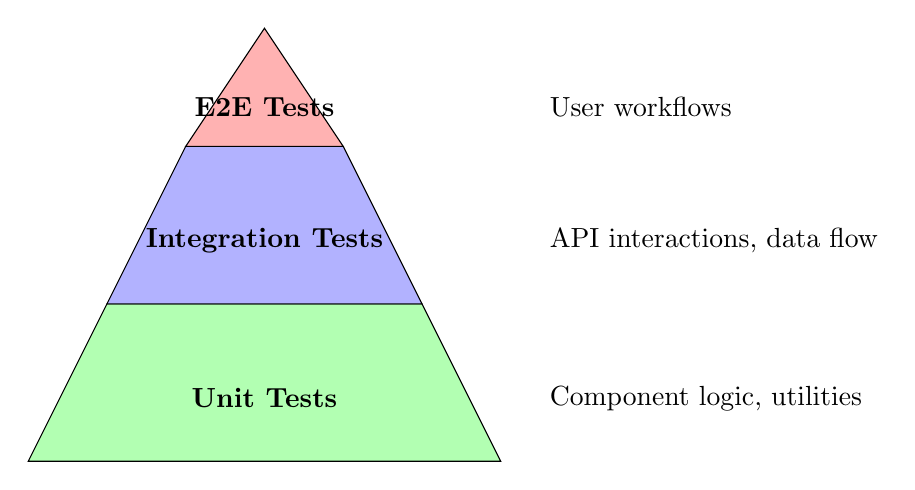
\begin{tikzpicture}
\draw[fill=green!30] (0,0) -- (6,0) -- (5,2) -- (1,2) -- cycle;
\draw[fill=blue!30] (1,2) -- (5,2) -- (4,4) -- (2,4) -- cycle;
\draw[fill=red!30] (2,4) -- (4,4) -- (3,5.5) -- cycle;

\node at (3,0.8) {\textbf{Unit Tests}};
\node at (3,2.8) {\textbf{Integration Tests}};
\node at (3,4.5) {\textbf{E2E Tests}};

\node[right] at (6.5,0.8) {Component logic, utilities};
\node[right] at (6.5,2.8) {API interactions, data flow};
\node[right] at (6.5,4.5) {User workflows};
\end{tikzpicture}
\caption{Testing Strategy Pyramid}
\end{figure}

\subsection{Test Coverage Goals}

\begin{table}[H]
\centering
\caption{Test Coverage Targets}
\begin{tabular}{@{}lll@{}}
\toprule
\textbf{Component Type} & \textbf{Target Coverage} & \textbf{Priority} \\
\midrule
Backend Functions & 90\% & High \\
React Components & 80\% & High \\
Utility Functions & 95\% & High \\
UI Components & 70\% & Medium \\
Integration Flows & 85\% & High \\
\bottomrule
\end{tabular}
\end{table}
